\documentclass{beamer}
\usetheme{Madrid}
\usecolortheme{default}

\title{Fundamentals of Perpetual Future}
\subtitle{Paper Review (Reviewer : Soowan Kim)}
\author{Songrun He, Asaf Manela, Omri Ross, Victor von Wachter}
\date{April 2023}

\logo{
\includegraphics[height=0.8cm]{snu_logo.png}}
\definecolor{uoftblue}{RGB}{6,41,88}
\setbeamercolor{titlelike}{bg=uoftblue}
\setbeamerfont{title}{series=\bfseries}
\renewcommand{\indent}{\hspace*{2em}}
\setbeamertemplate{caption}{\raggedright\insertcaption\par}

\begin{document}

\frame{\titlepage}

\begin{frame}
\frametitle{Table of Contents}
\tableofcontents
\end{frame}

\section{Research Question}

\begin{frame}
\frametitle{Research Question}
1. What are the theoretical fundamental values of perpetual future.\\~\\
2. How large are deviations from these fundamentals empirically.\\~\\
3. What causes this deviations.
\end{frame}

\section{Perpetual Futures}

\begin{frame}
\frametitle{Perpetual Futures}
\begin{block}{Definition}
~Bilateral agreements that the party on the short side is required to pay the long side a sum based on the \alert{increase in the futures price} between when they enter and exit the contract.
Meanwhile, the long side pays the short side an ongoing cash flow called the \alert{“funding rate”}.
\end{block}
\end{frame}

\begin{frame}
\begin{itemize}
    \item Purpose
    \begin{itemize}
        \item Original Idea\\~Enable price discovery for the underlying with an illiquid or hard-to-measure price. 
        \item Crypto Market\\~Offer an effective leveraged trading vehicle to hedge or speculate the underlying spot price movement, making the market more complete.
    \end{itemize}
    ~\\
    \item Pros \& Cons
    \begin{itemize}
        \item Improves the liquidity of the contract.
        \item No need to rollover.
        \item Not guaranteed to converge to the spot.
    \end{itemize}
\end{itemize}
\end{frame}

\section{Perpetual Futures Pricing}

\begin{frame}
\frametitle{Perpetuals Pricing}
\begin{block}{Definition 1. Perpetual Future}
~Notate perpetual future written on $\{S_t\}_{t=0}^\infty$ as $\{F_t\}_{t=0}^\infty$. There is 0 cost to enter the agreement and both the long side and the short side can terminate the contract at any time t. \\~Before termination, for each unit of perpetual future, the long must pay the short an $\mathcal{F}_s-$adapted cash-flow \alert{$\kappa(F_s-S_s)ds $}$,s \in (0, t)$, referred to as the funding value. $\kappa$ is a scaling parameter determining the magnitude of the funding rate relative to the price gap. At termination, the short needs to pay the long \alert{$F_t-F_0$} for each unit shorted.
\end{block}
~This definition is an approximation of real-world perpetual futures. If we measure time units in years, this setup would correspond to $\kappa = 1095$.
\end{frame}

\begin{frame}
\frametitle{Perpetuals Pricing}
$\kappa(F_s-S_s)ds$\\~\\
~The definition is assuming the funding value to be approximately proportional to the difference between the futures price and the spot. 
\begin{figure}
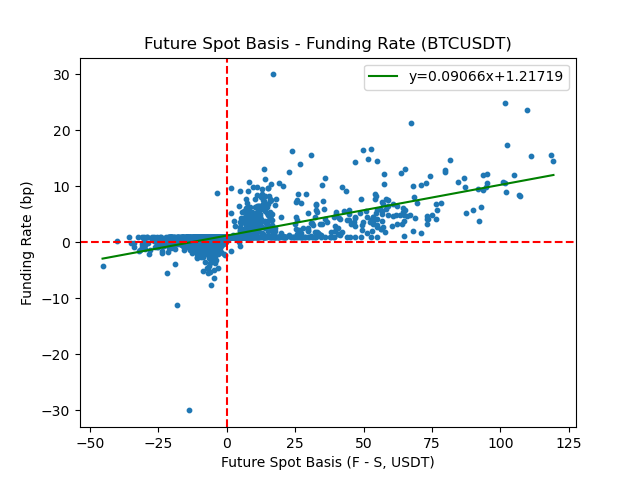
\includegraphics[scale=0.35]{figs/Future Spot Basis - Funding Rate/Future Spot Basis - Funding Rate (BTCUSDT).png}
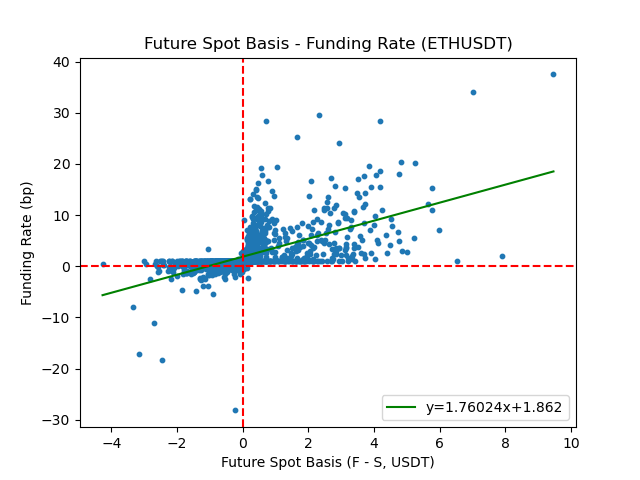
\includegraphics[scale=0.35]{figs/Future Spot Basis - Funding Rate/Future Spot Basis - Funding Rate (ETHUSDT).png}
\end{figure}
\end{frame}

\begin{frame}
\frametitle{Perpetuals Pricing}
\begin{block}{Definition 2. Traditional Arbitrage}
~A (riskless) arbitrage opportunity is defined with respect to payoff $x$ at a \alert{certain future time t} and its price $p(x)$. This payoff is an arbitrage opportunity if the following conditions are satisfied: \\~(1) $x \geq 0$ almost surely, (2) $x > 0$ with some positive probability, and (3) its price satisfies $p(x) \leq 0$.
\end{block}
\begin{block}{Definition 3. Random Maturity Arbitrage}
A random-maturity arbitrage opportunity is defined with respect to a random payoff x at a \alert{future random time $\tilde\tau \in (0,\infty)$}, and its price $p(x)$. This payoff is a random-maturity arbitrage opportunity if the following conditions are satisfied:\\~(1) $x\geq0$ almost surely, (2) $x>0$ with some positive probability, and (3) its price satisfies $p(x)\leq0$.
\end{block}
\end{frame}

\begin{frame}
\frametitle{Perpetuals Pricing}
\begin{alertblock}{Corollary 1.}
~In the perpetual futures market, if a strategy has \\ \begin{enumerate}[i]
    \item 0 cost at time 0
    \item for any price path of the futures and the spot$\{F_t\}_{t=0}^\infty$ and $\{S_t\}_{t=0}^\infty$ there exists an unwinding time $\tilde t$ such that its discounted payoff at time $t = \tilde t$ is positive
\end{enumerate} 
then this strategy is a random-maturity arbitrage.
\end{alertblock}
\end{frame}

\begin{frame}
\frametitle{Perpetuals Pricing}
\begin{block}{Assumption 1.}
~The gap between the perpetual futures and the spot satisfies the following condition: $\liminf_{t\to\infty}|F_t(\omega)-S_t(\omega)| < \infty, \forall \omega$
\end{block}
~\\
\begin{block}{Assumption 2.}
~The risk-free rate $r$ for arbitrageurs is constant.
\end{block}
\end{frame}

\begin{frame}
\frametitle{Perpetuals Pricing}
\begin{alertblock}{Proposition 1. No-arbitrage bound}
~Under Assumptions 1 and 2, when there is a constant trading cost $C$ when terminating the position, arbitrageurs will trade the perpetual futures until it lies within a bound of the spot:$$S_t(1+\frac{r}{\kappa})-C\leq F_t\leq S_t(1+\frac{r}{\kappa})+C$$
\end{alertblock}
\begin{alertblock}{Proposition 2. No-arbitrage price}
~When there is no trading cost (C = 0), arbitrageurs will trade perpetual futures toward: $$F_t = S_t\left(1+\frac{r}{\kappa}\right)$$
\end{alertblock}
~\\
\end{frame}

\begin{frame}
\frametitle{Perpetuals Pricing}
\begin{figure}
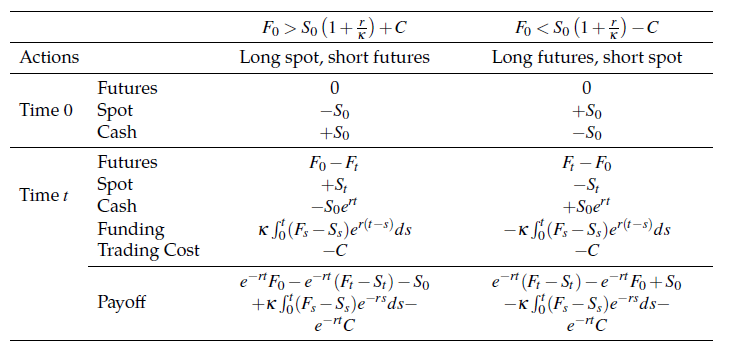
\includegraphics[scale=0.8]{figs/Table1.png}
\end{figure}
~In the first scenario, to ensure that the stated strategy avoids any random-maturity arbitrage opportunities:
\begin{figure}
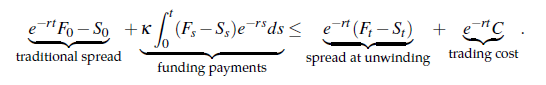
\includegraphics[scale=0.9]{figs/Equation(2).png}
\end{figure}
\end{frame}

\begin{frame}
\frametitle{Perpetuals Pricing}
\begin{figure}
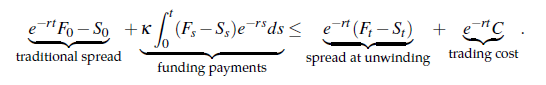
\includegraphics[scale=0.95]{figs/Equation(2).png}
\end{figure}
~Denote $(F_t-S_t)e^{-rt}\equiv u_t$, $$u_t\geq e^{-rt}(F_0-C)-S_0+\kappa\int_0^t u_sds.$$
~$\underbar u_t = e^{-rt}(F_0-C)-S_0+\kappa\int^t_0 \underbar u_s ds$ provides a lower bound for all processes $u_t$ satisfying the above inequality. Solving this integral equation, we have: $$\underbar u_t=\frac{F_0r_e^{-rt}}{\kappa+r}+\left(\frac{F_0-c}{1+\frac{r}{\kappa}}-S_0\right)e^{\kappa t}.$$
~When $F_0>S_0(1+\frac{r}{\kappa})+C$, $\lim_{t\to\infty}\underbar u_t=\infty$. This contradicts Assumption 1, and therefore, when $F_0 > S_0(1+\frac{r}{\kappa})+C$, longing the spot and shorting the futures would be a random-maturity arbitrage opportunity.
\end{frame}

\begin{frame}
\frametitle{Perpetuals Pricing}
Q. Is it appropriate to generalize notion of (riskless) arbitrage like this?
\begin{block}{Definition 3. Random Maturity Arbitrage}
A random-maturity arbitrage opportunity is defined with respect to a random payoff x at a \alert{future random time $\tilde\tau \in (0,\infty)$}, and its price $p(x)$. This payoff is a random-maturity arbitrage opportunity if the following conditions are satisfied:\\~(1) $x\geq0$ almost surely, (2) $x>0$ with some positive probability, and (3) its price satisfies $p(x)\leq0$.
\end{block}
Maybe too \alert{generous} to call this definition \textit{riskless}. \\\quad e.g.) risk of the position being underwater for a considerably long period before finally turning positive. \\\quad Note that the high liquidation risk of perpetuals in the crypto market, due to its high volatility, will increase significantly as the holding period gets longer.
~\\
\end{frame}

\section{Empirical Analysis}

\begin{frame}
\frametitle{Data}
For major crypto-currencyies of BTC, ETH, BNB, DOGE, ADA,\\~\\
\begin{table}
\footnotesize
\begin{tabular}{l | c | c | c | c | c}
Data & Freq & Start & End & Source & Notes\\
\hline \hline
Spot \& Future & 1h & 2019.09.10 & 2022.11.13 & Binance(A) & \\ 
Funding Rate & 8h & 2019.09.10 & 2022.11.13 & Binance(A) &\\
Trading Cost & n/a & n/a & n/a & Binance(A) & \\
Interest Rate & 1d & 2020.01.08 & 2022.11.13 & Aave(A) & \tiny AVG(USDT,USDC,DAI)\\
fear\&greed idx & n/a & n/a & n/a & \tiny alternative.me(A) & [0,100]\\
\end{tabular}
\end{table}
\end{frame}

\begin{frame}
\frametitle{Data}
\begin{figure}
    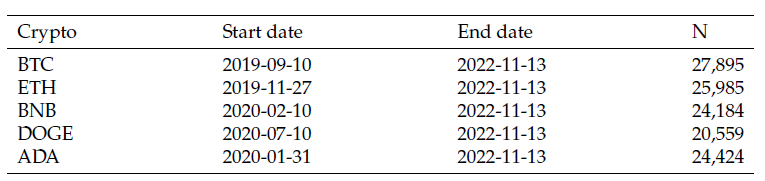
\includegraphics[scale=0.8]{figs/Table2.png}
    \caption{Perpetual Futures \& Spot price (1h, Binance)}
        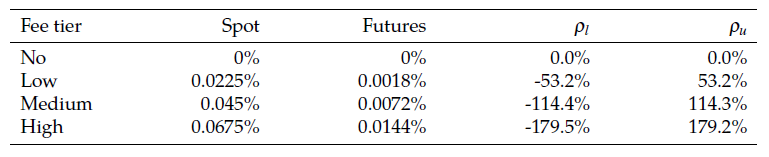
\includegraphics[scale=0.8]{figs/Table3.png}
    \caption{Trading costs specifications}
\end{figure}
\end{frame}

\begin{frame}
\frametitle{Deviations of perpetuals from no-arbitrage benchmarks}
Annualized Deviation $\rho$ \\: Defined as the interest rate that rationalizes an observed future-spot spread$$F=S\left(1+\frac{r+\rho}{\kappa}\right)$$~\\~Using $f$ and $s$ to denote $log(F)$ and $log(S)$ respectively, $$\rho=\kappa(f-s)-r$$
\end{frame}

\begin{frame}
\frametitle{Deviations of perpetuals from no-arbitrage benchmarks}
\begin{figure}
    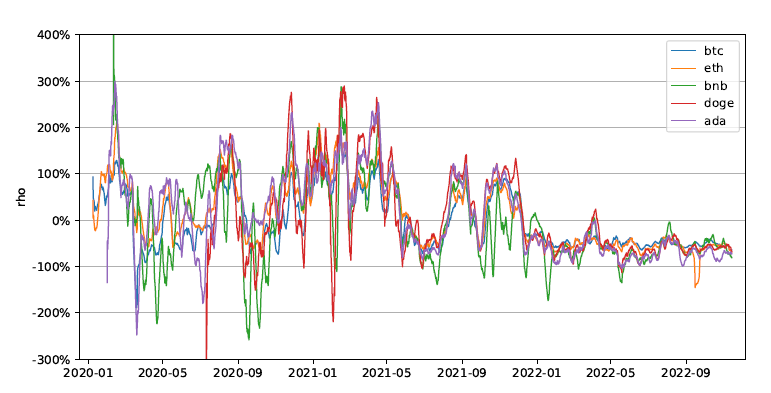
\includegraphics[width=0.75\linewidth]{figs/Figure3.png}
\end{figure}
~After the year 2022, futures-spot spreads become smaller in magnitude and less volatile compared to earlier years, staying around -50\%.
\begin{enumerate}[i]
    \item The market is becoming increasingly efficient.
    \item Relative demand in futures market is weaker compared to the spot.
    \item Due to lack of infrastructure to short the cryptos in the spot market, arbitrageur's funding constraints are larger in the negative region.
\end{enumerate}
\end{frame}

\begin{frame}
\frametitle{Deviations of perpetuals from no-arbitrage benchmarks}
\begin{figure}
    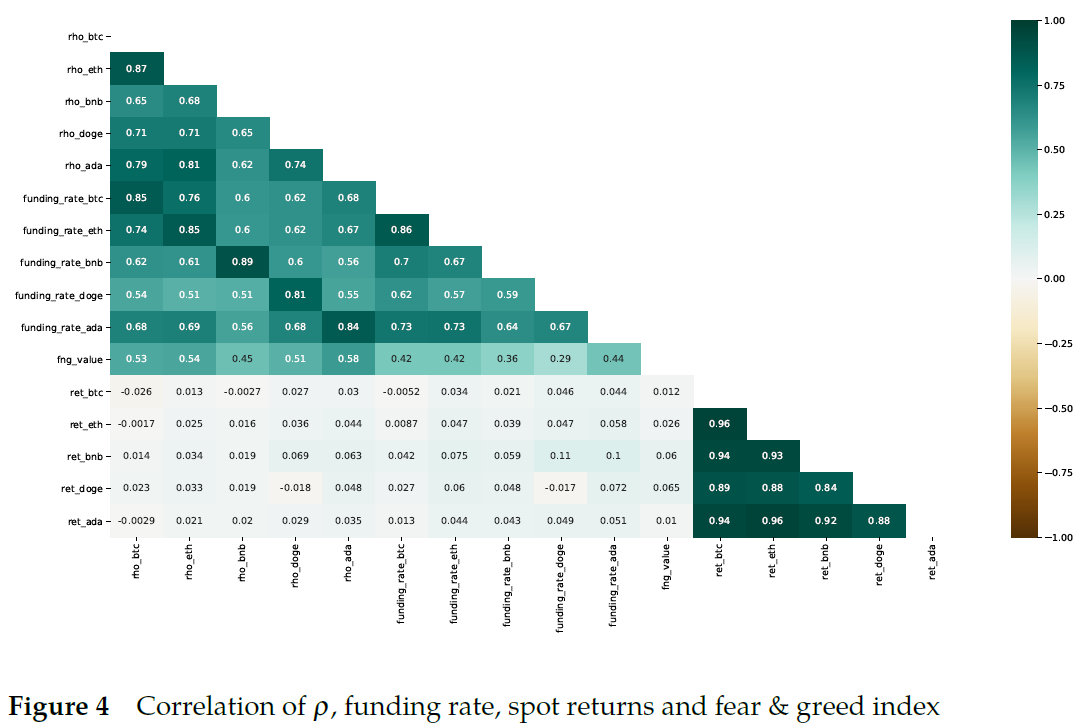
\includegraphics[width=0.95\linewidth]{figs/Figure4.png}
\end{figure}
\end{frame}

\begin{frame}
\frametitle{Deviations of perpetuals from no-arbitrage benchmarks}
\begin{itemize}
    \item Significant comovement in futures-spot spreads across all five cryptocurrencies.\\~\\
    \item Correlation between deviations $\rho$ and spot market returns is low.\\~\\
    \item $\rho$ highly correlated with the funding rate.
\end{itemize}
\end{frame}

\begin{frame}
\frametitle{Random-maturity Arbitrage Strategy}
\begin{figure}
    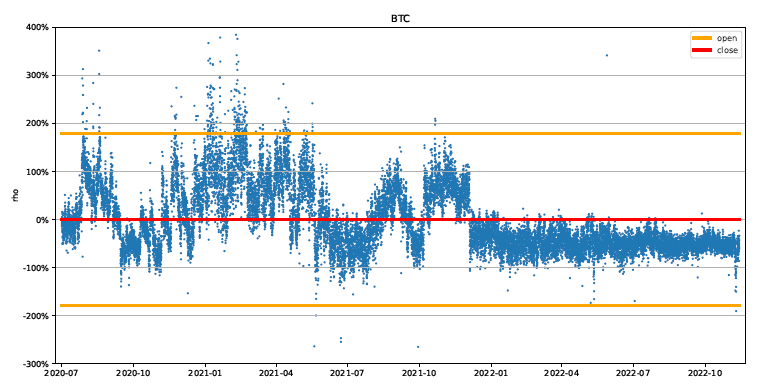
\includegraphics[width=0.75\linewidth]{figs/Figure5.png}
\end{figure}
\end{frame}

\begin{frame}
\frametitle{Random-maturity Arbitrage Strategy}
Sharpe Ratio Calculation
\begin{enumerate}[i]
    \item Calculate the mean ($\mu$) and standard deviation ($\sigma$) of our trading strategy during the time it is active. 
    \item Scale $\mu/\sigma$ by the number of periods the strategy is active in a year: $$SR=\frac{\mu}{\sigma}\sqrt{N_a}$$ where $\mu$ and $\sigma$ are average hourly returns and $N_a$ is the average number of hours the strategy is active in a year.
\end{enumerate}
\end{frame}

\begin{frame}
\frametitle{Random-maturity Arbitrage Strategy}
Yields highly significant alphas unexplained by previous risk factors.
\begin{figure}
    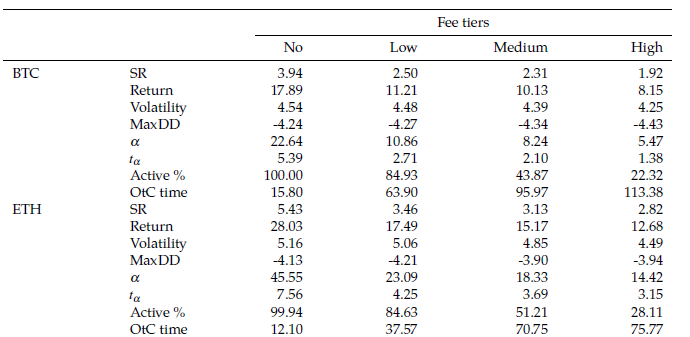
\includegraphics[width=0.65\linewidth]{figs/Table4-1.png}
    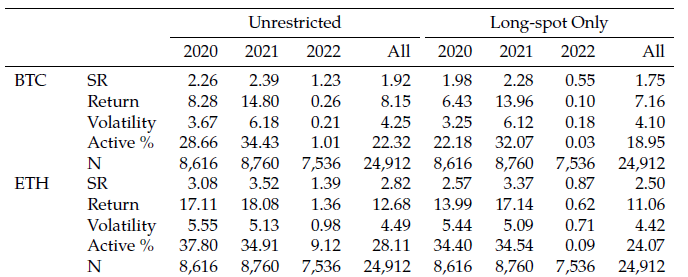
\includegraphics[width=0.65\linewidth]{figs/Table5-1.png}
\end{figure}
\end{frame}

\begin{frame}
\frametitle{Random-maturity Arbitrage Strategy}
Two main sources of gains: 
\begin{enumerate}
    \item Price convergence
    \item Funding rate payments
\end{enumerate}
\begin{figure}
    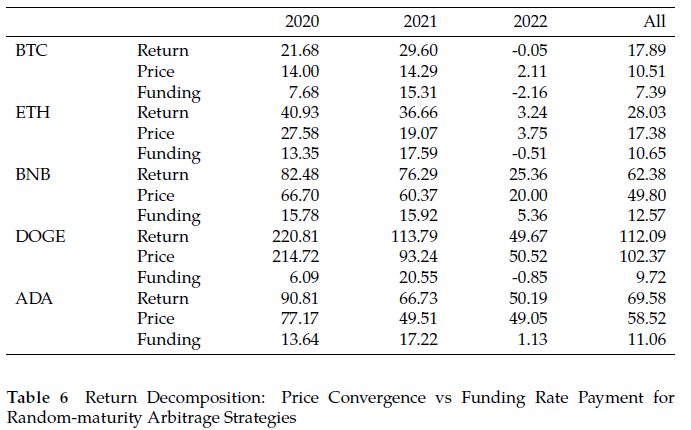
\includegraphics[width=0.65\linewidth]{figs/Table6.png}
\end{figure}
Price convergence plays a dominant role while funding rate payments have a more minor role, which seems to \textit{diminish over time}.
\end{frame}

\section{Explaining Futures-spot Deviations}

\begin{frame}
\frametitle{Comovement of futures-spot deviation across crypto assets}
\begin{description}
    \item[Hypothesis 1] Reflects \alert{time-varying funding constraints} experienced by arbitrageurs in the market.
    \item[Hypothesis 2] \alert{Commonality in sentiment} across different cryptocurrencies from the demand side.
\end{description}
~\\Proxies
\begin{itemize}
    \item H1 : Past Returns \\(for relative extrapolative demand in the perpetual futures market compared to the spot market)
    \item H2 : Crypto Return Volatility \\(arbitrageurs likely face Value-at-Risk (VaR) type constraints, which are more likely to bind when market volatility is high)
\end{itemize}
\end{frame}

\begin{frame}
\frametitle{Comovement of futures-spot deviation across crypto assets}
\begin{figure}
    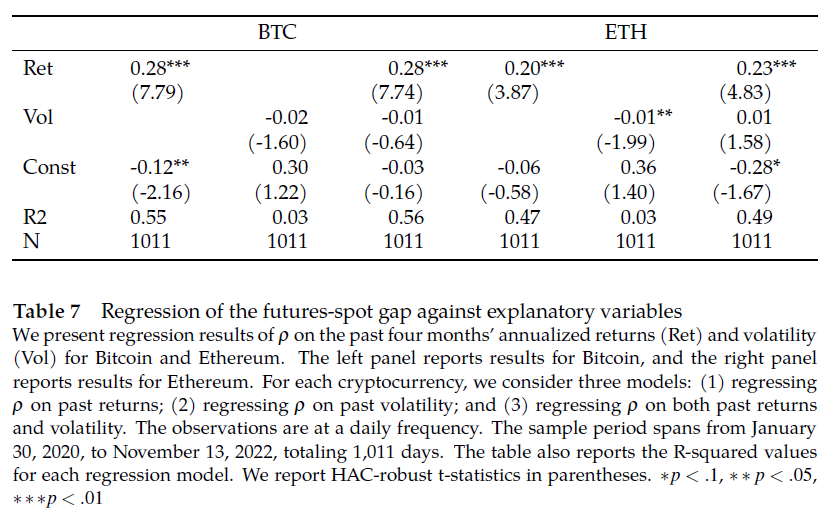
\includegraphics[width=0.8\linewidth]{figs/Table7.png}
\end{figure}
\end{frame}

\begin{frame}
\frametitle{Comovement of futures-spot deviation across crypto assets}
\begin{itemize}
    \item When past returns are high, perpetual futures exhibit a more positive deviation against the spot.
    \item Volatility does not significantly covary with the futures and spot deviation.
\end{itemize}
~\\Market Mechanism
\begin{itemize}
    \item \alert{Arbitrage trading} will accommodate all the demand in the futures until the price deviation \textit{lies within a trading cost bound.}
    \item \alert{Relative demand of futures}, compared to the spot still \textit{manifest itself within the bound} in the deviation of futures prices from the spot.\\~Due to the comovement of the time-varying relative demand, we observe a significant common factor in crypto future-spot deviations.
\end{itemize} 
\end{frame}

\end{document}